% --------------------------------------------------------------
% This is all preamble stuff that you don't have to worry about.
% Head down to where it says "Start here"
% --------------------------------------------------------------
 
\documentclass[12pt]{article}

\usepackage{courier}
\usepackage{color}
\usepackage{listings}
\usepackage[square,numbers]{natbib}
\usepackage{tabls}
\usepackage{graphicx}
\usepackage{subcaption}
\usepackage{pdfpages}
\usepackage{mathtools}

\definecolor{dkgreen}{rgb}{0,0.6,0}
\definecolor{gray}{rgb}{0.5,0.5,0.5}




\lstset{language=Matlab,
   keywords={break,case,catch,continue,else,elseif,end,for,function,
      global,if,otherwise,persistent,return,switch,try,while},
   basicstyle=\ttfamily,
   keywordstyle=\color{blue},
   commentstyle=\color{red},
   stringstyle=\color{dkgreen},
   numbers=left,
   numberstyle=\tiny\color{gray},
   stepnumber=1,
   numbersep=10pt,
   backgroundcolor=\color{white},
   tabsize=4,
   showspaces=false,
   showstringspaces=false}
 
\usepackage[margin=1in]{geometry} 
\usepackage{amsmath,amsthm,amssymb}
\usepackage{verbatim}
\usepackage{algpseudocode,algorithm}
\usepackage{setspace}

\newcommand{\lline}{\noindent\makebox[\linewidth]{\rule{\textwidth}{0.4pt}}}
\newcommand{\N}{\mathbb{N}}
\newcommand{\Z}{\mathbb{Z}}
\newcommand{\deriv}[2]{\frac{\mathrm{d} #1}{\mathrm{d} #2}}
\newcommand{\pderiv}[2]{\frac{\partial #1}{\partial #2}}
\newcommand{\bx}{\mathbf{X}}
\newcommand{\ba}{\mathbf{A}}
\renewcommand{\d}{\mathrm{d}}
\newcommand{\upl}{u_{\text{plane}}}
\newcommand{\upt}{u_{\text{point}}}
\newcommand{\D}{\Delta}
\newcommand{\ra}{\rightarrow}
\renewcommand{\SS}{\State}
 
\newenvironment{theorem}[2][Theorem]{\begin{trivlist}
\item[\hskip \labelsep {\bfseries #1}\hskip \labelsep {\bfseries #2.}]}{\end{trivlist}}
\newenvironment{lemma}[2][Lemma]{\begin{trivlist}
\item[\hskip \labelsep {\bfseries #1}\hskip \labelsep {\bfseries #2.}]}{\end{trivlist}}
\newenvironment{exercise}[2][Exercise]{\begin{trivlist}
\item[\hskip \labelsep {\bfseries #1}\hskip \labelsep {\bfseries #2.}]}{\end{trivlist}}
\newenvironment{problem}[2][Problem]{\begin{trivlist}
\item[\hskip \labelsep {\bfseries #1}\hskip \labelsep {\bfseries #2:}]\hspace{0.3in}\newline\newline}{\end{trivlist}}
\newenvironment{question}[2][Question]{\begin{trivlist}
\item[\hskip \labelsep {\bfseries #1}\hskip \labelsep {\bfseries #2.}]}{\end{trivlist}}
\newenvironment{corollary}[2][Corollary]{\begin{trivlist}
\item[\hskip \labelsep {\bfseries #1}\hskip \labelsep {\bfseries #2.} ]}{\end{trivlist}}
\newenvironment{problem*}[1][Problem]{\begin{trivlist}
\item[\hskip \labelsep {\bfseries #1} {\hspace{-0.2em}\bfseries:}]}{\end{trivlist}}
\newenvironment{solution}[1][Solution]{\begin{trivlist}
\item[\hskip \labelsep {\bfseries #1} {\hspace{-0.2em}\bfseries:}]\hspace{0.3in}\newline}{\end{trivlist}}
 
\begin{document}
 
% --------------------------------------------------------------
%                         Start here
% --------------------------------------------------------------
 
\title{Homework 1}%replace X with the appropriate number
\author{Simon Bolding\\ %replace with your name
NUEN 629} %if necessary, replace with your course title
 
\maketitle

\clearpage

%\includepdf[pages={1}]{p1p3.pdf}

\begin{problem}{1}
Henyey and Greenstein (1941) introduced a function which, by the variation of one
parameter, $−1 \leq h \leq 1$, ranges from backscattering through isotropic scattering to forward scattering. In
our notation we can write this as
\begin{equation}
    K( \mu_0 , v'\rightarrow v) = \frac{1}{2}
    \frac{1-h^2}{\left(1+h^2-2h\mu_0\right)^{3/2}}\delta(v'-v).
\end{equation}
Verify that this is a properly normalized $f ( \mu_0 )$ and compute $K_l (v'
\rightarrow → v)$ for $l = 0, 1, 2$ as a function of $h$.

\end{problem}

\begin{solution}
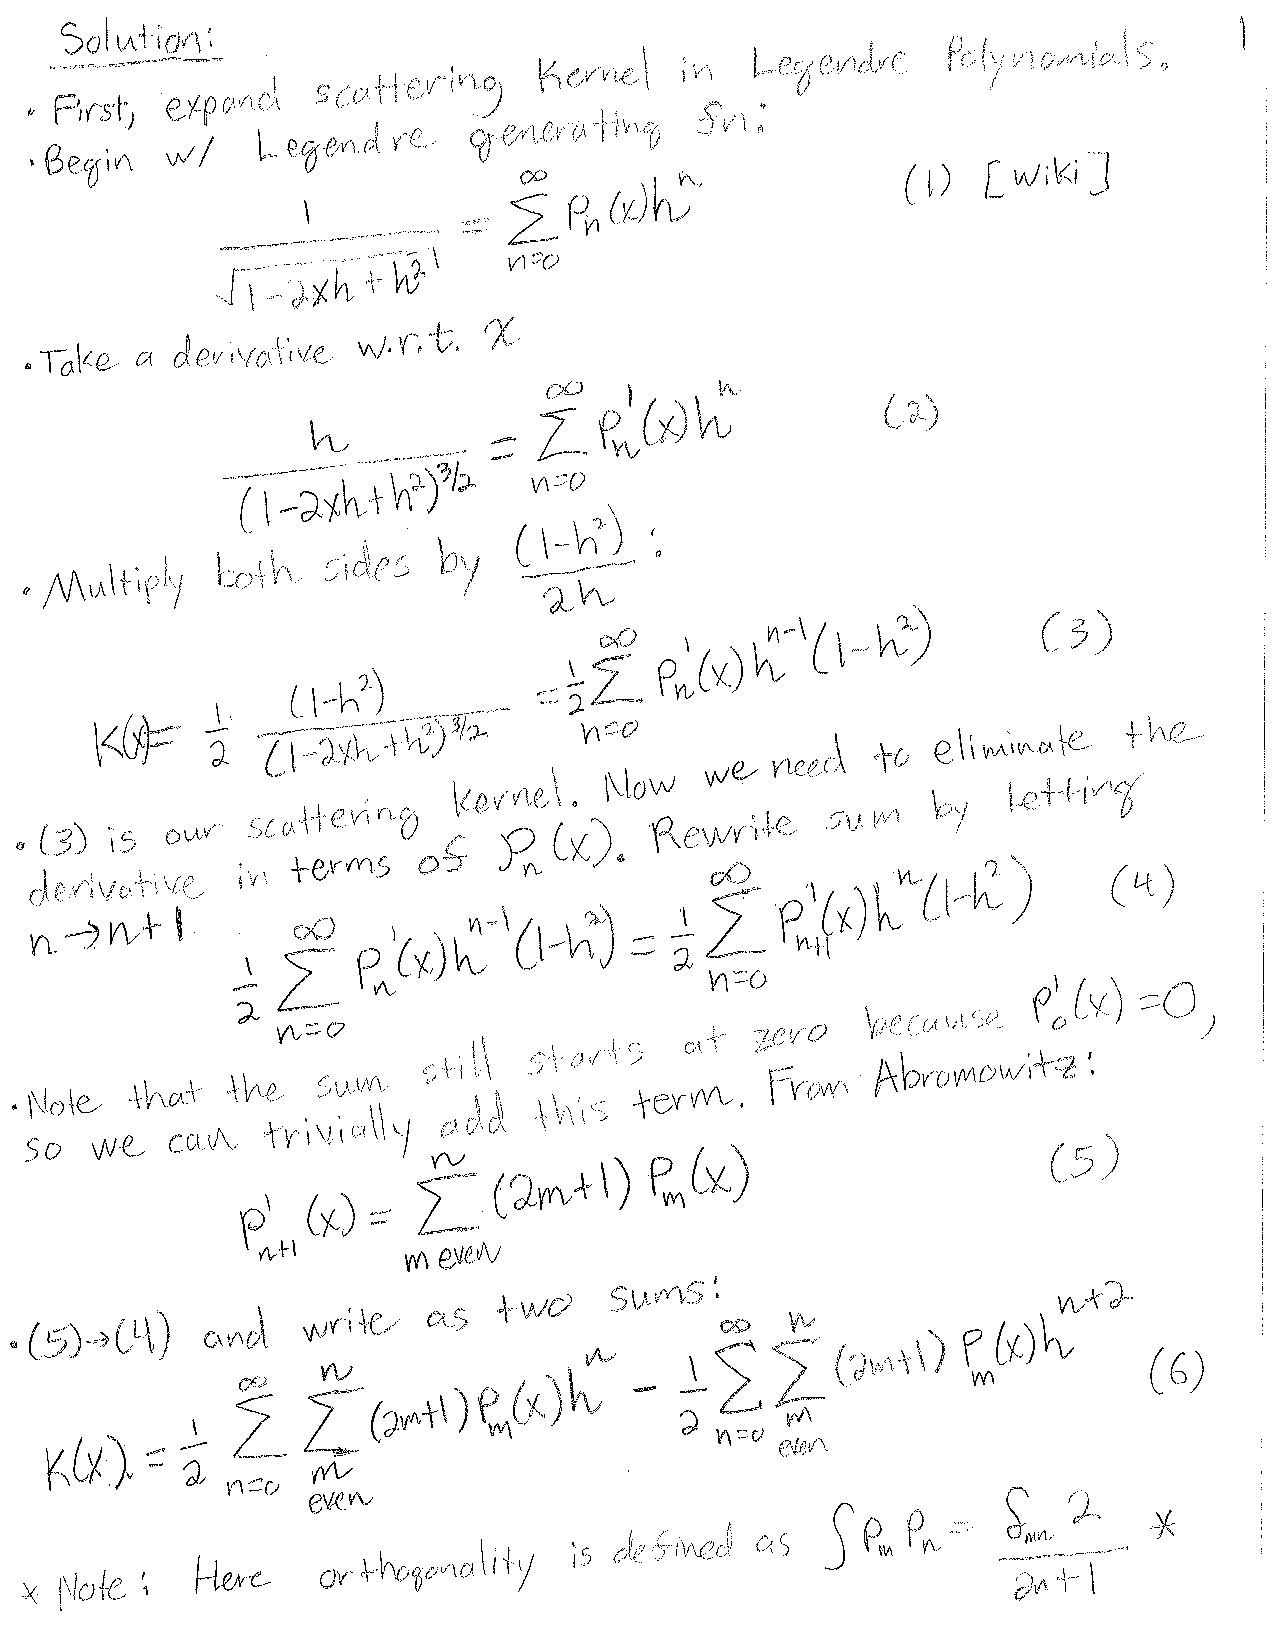
\includepdf[pages={1-2}]{p1.pdf}
\end{solution}
\clearpage

\begin{problem}{2}
In an elastic scatter between a neutron and a nucleus, the scattering angle in the center of mass system is
related to the energy change as
\begin{equation}\label{eq:E}
 \frac{E}{E'} = \frac{1}{2}\left((1+\alpha) + (1-\alpha)\cos \theta_c\right)
\end{equation}
where $E$ is the energy after scattering and $E'$′ is the initial energy of the neutron and
\begin{equation}
\alpha = \frac{(A-1)^2}{(A+1)^2}.
\end{equation}
The scattered angle in the center-of-mass system is related the lab-frame scattered angle as
\begin{equation}
\tan \theta_L = \frac{A\sin \theta_c}{1 + A\cos \theta_c}
\end{equation}
Also, the distribution of scattered energy is given by
\begin{equation} \label{pdf}
P(E'\rightarrow E) = \left\{\begin{matrix}
\frac{1}{(1-\alpha)E'} & E'\alpha \leq E \leq E' \\ 
 0 & \text{otherwise}
\end{matrix}\right. .
\end{equation}
Derive an expression for $K( \mu_0, E'\rightarrow E)$, where $\mu_0$ is $\cos \theta_L$. What is the distribution in angle of neutrons of energy
in the range [0.05 MeV, 10 MeV] to energies below 1 eV if the scatter is with hydrogen?

\end{problem}

\begin{solution}
Due to Eq.~\eqref{eq:E}, for a fixed $A$, a given value of $E$ and $E'$ fully define
$\mu_c$. As a result, the shape of the doubly differential scattering cross section
 in the center of mass (COM) system is fully defined by the probability density function (PDF) $P(E'\ra E)$. Thus, it is
possible to write the scattering cross section in the COM frame as~\cite{dunnshultis}
\begin{equation}
    \Sigma_s(E,\mu_0) = \sigma_S(E')(P(E' \ra E) \delta(\mu_c - f(E,E'))
 \end{equation}
 where $f(E,E')$ is the value of $\mu_c$ that satisfies Eq.~\eqref{eq:E} for a given
 $E$, i.e.,
 \begin{equation}
     f(E,E') = 
 \end{equation}
 Since we are interested in s, we only need to transform the PDF $P(E'\ra E)$ into a density function
 $P(\mu_0)$. From Eq.~\eqref{Eq:E},
 there is a one-to-one relationship between $E$ and $\mu_c=\cos(\Theta_c)$, thus 
 \begin{equation}
  P(E'\ra E) \d E = P(\mu_c)\d \mu_C.
 \end{equation}
 or
 \begin{equation} \label{pdfmu}
  P(\mu_c) = P(E' \ra E) \frac{\d E}{\d \mu_c}.
 \end{equation}
 Differentation of Eq.~\eqref{eq:E} and multiplication by $E'$ yields
 \begin{equation}
     \frac{ \d E}{\d \mu_c} = \frac{1}{2}(1-\alpha) E'
 \end{equation}
 Evaluating $\mu_c$ for $E$ at the limits $\alpha E'$
 and $E'$ gives the support for $P(\mu_c)$, defined for $\mu_c \in[ -1,1 ]$.  
 Substitution of the above equation and Eq.~\eqref{pdf} into Eq.~\eqref{pdfmu} gives
 the desired PDF
 \begin{equation}
     P(\mu_c) = \frac{1}{(1-\alpha)E'} \left( \frac{1}{2}(1-\alpha)E' \right) =
     \frac{1}{2}, \quad \mu \in [-1,1]
 \end{equation}
 




 \end{solution}

 \begin{thebibliography}{9}

     \bibitem{dunnshultis}
         W.L. Dunn and J.K. Shultis, \emph{Exploring Monte Carlo Methods}, 2012.


\end{thebibliography}

\end{document}



